\documentclass[review]{elsarticle}
\usepackage[margin=1in]{geometry}
\usepackage{lineno,hyperref}
\usepackage{mathtools}
\usepackage{amsfonts}
\usepackage[utf8]{inputenc}
\usepackage[english]{babel}
\usepackage{subfig}
\usepackage{hyperref}
\usepackage{amsmath}
\hypersetup{
    colorlinks=true,
    linkcolor=blue,
    filecolor=magenta,      
    urlcolor=cyan,
}

\DeclarePairedDelimiter{\ceil}{\lceil}{\rceil}
\modulolinenumbers[5]
\journal{Journal of \LaTeX\ Templates}

%%%%%%%%%%%%%%%%%%%%%%%
%% Elsevier bibliography styles
%%%%%%%%%%%%%%%%%%%%%%%
%% To change the style, put a % in front of the second line of the current style and
%% remove the % from the second line of the style you would like to use.
%%%%%%%%%%%%%%%%%%%%%%%

%% Numbered
%\bibliographystyle{model1-num-names}

%% Numbered without titles
%\bibliographystyle{model1a-num-names}

%% Harvard
%\bibliographystyle{model2-names.bst}\biboptions{authoryear}

%% Vancouver numbered
%\usepackage{numcompress}\bibliographystyle{model3-num-names}

%% Vancouver name/year
%\usepackage{numcompress}\bibliographystyle{model4-names}\biboptions{authoryear}

%% APA style
%\bibliographystyle{model5-names}\biboptions{authoryear}

%% AMA style
%\usepackage{numcompress}\bibliographystyle{model6-num-names}

%% `Elsevier LaTeX' style

\bibliographystyle{elsarticle-num}

%Macros
\def\github{https://github.com/walkanth/pysweep}
\def\oldCPU{s}
\def\oldGPU{s}
\def\newCPU{s}
\def\newGPU{s}

%%%%%%%%%%%%%%%%%%%%%%%
%----------------MACROS--------------------
\def\github{\url{https://github.com/anthony-walker/pysweep-git}}

\def\pysweep{\texttt{PySweep}}
\def\Swept{\texttt{Swept}}
\def\Standard{\texttt{Standard}}
\def\Up{\texttt{Up-Pyramid}}
\def\Down{\texttt{Down-Pyramid}}
\def\Oct{\texttt{Octahedron}}
\def\Xb{\texttt{X-Bridge}}
\def\Yb{\texttt{Y-Bridge}}

\def\oldCPU{Intel Skylake Silver 4114} %20 core cpu
\def\oldGPU{Nvidia GeForce GTX 1080 Ti}

\def\newCPU{Intel E5-2698v4} %20 core cpu
\def\newGPU{Tesla V100-DGXS-32GB}


\begin{document}

\begin{frontmatter}

\title{The 2-Dimensional Swept Rule Applied on Heterogeneous Architecture}

%% Group authors per affiliation:
\author{Anthony Walker, Dr. Kyle Niemeyer\fnref{myfootnote}}
% \address{Radarweg 29, Amsterdam}
% \fntext[myfootnote]{Since 1880.}

%% or include affiliations in footnotes:
% \author[mymainaddress,mysecondaryaddress]{Elsevier Inc}
% \ead[url]{www.elsevier.com}

% \author[mysecondaryaddress]{Global Customer Service\corref{mycorrespondingauthor}}
% \cortext[mycorrespondingauthor]{Corresponding author}
% \ead{walkanth@oregonstate.edu}
%
% \address[mymainaddress]{1600 John F Kennedy Boulevard, Philadelphia}
% \address[mysecondaryaddress]{360 Park Avenue South, New York}



\begin{abstract}
This paper contain is a study of the swept rule in two dimensions on heterogeneous architecture.


\end{abstract}

\begin{keyword}
\texttt{elsarticle.cls}\sep \LaTeX\sep Elsevier \sep template
\MSC[2010] 00-01\sep  99-00
\end{keyword}

\end{frontmatter}

\linenumbers

\section{Introduction}
Partial differential equations (PDEs) are used to model many phenomena in science and engineering. Fluid mechanics and heat transfer are among these phenomena which can be notoriously difficult to solve on a pragmatic scale. Wildfire is a good example of this because it involves fluid mechanics, heat transfer, and chemistry over massive areas of impact. Wildfire is also an unsteady phenomenon---so it changes over time. The ability to accurately model and predict the properties of such a phenomenon in real time would allow for better response to it but there are many challenges associated with making these predictions.

Unsteady multidimensional PDEs often require the use of distributed memory systems to obtain a solution with practical grid resolution or scale in a reasonable time frame. The solution of many problems at any point in the grid is inherently dependent on the neighboring points in each dimension. This dependence necessitates communication between computing nodes. Each of these communications incurs a minimum cost regardless of the amount of information communicated known as network latency. On the contrary, bandwidth is the variable cost associated with the amount of data transferred. This latency can be significantly restrictive on the solution's time to completion, especially when using distributed systems. This barrier to scaling is referred to as the latency barrier and is impactful in large scale simulations advancing many time steps, i.e., ones that requires a large amount of communication \cite{Alhubail2016ThePDEs}. The barrier is a bottle neck in the system which can limit the performance regardless of the architecture.

\par
GPUs are powerful tools for scientific computing because they are highly suited for parallel applications and a lot of number crunching. Similar to nodes on a cluster, they perform best when as much work as possible is completed locally prior to communication. Heterogeneous system is a system with multiple processor types; A system with CPUs and GPUs in this case.  Ideally, a heterogeneous application will minimize communication between the GPU and CPU which effectively minimizes latency costs \cite{OanceaGPGPUCOMPUTING}. Minimizing latency in high performance computing (HPC) is one of the barriers to exascale computing which requires the implementation of novel techniques to improve \cite{Alexandrov2016RouteSkills}.

\par
In this article we describe the implementation and performance of a two dimensional heterogeneous solver for unsteady partial differential equations, \pysweep{}\footnote{\github}, that employs a technique to help overcome the latency barrier---the swept rule. We first discuss related work, the difference of our work, and more motivation in section~\ref{related-section}. Next, we describe some implementation details, objectives, study parameters, design decisions, methods, and tests in section~\ref{methods-section}. As expected, this is followed with results and conclusions in sections~\ref{results-section} and~\ref{conclusions-section}. Finally, the paper closes with acknowledgements, references, and appendices.

\section{Related Work}
\label{related-section}
\par The latency barrier has been approached in many ways; the most closely related to this study being other swept rule studies which involve multiple dimensions and architectures but not the combination of the two \cite{Alhubail2016ThePDEs,Alhubail2018ThePDEs,Magee2018AcceleratingDecomposition,Magee2020ApplyingSystems}. This technique is also related to parallel-in-time methods, cache optimization techniques, and communication avoidance (CA) algorithms but there are technical differences in each of the strategies.

\par
Parallel-in-time methods differ from the swept rule in the sense that it is not iterative and they are attempting to parallelize the temporal direction \cite{Gander201550Integration}. There are many examples of parallel-in-time methods such as multigrid-reduction-in-time, Parareal, adaptive Parareal, Parareal with local time integrators, PFASST, and interwoven PFASST with multigrid \cite{Falgout2014ParallelMultigrid,Lions2013Resolution,Maday2020AnAlgorithm,Wu2018Parareal,EmmettTowardEquations,MinionINTERWEAVINGMULTIGRID}. All of these methods are variations of the core concept of parallel in time methods. For example, Parareal is one of the more popular parallel-in-time methods; it works by iterating over a series of course and fine grids with initial guesses to parallelize the problem \cite{Lions2013Resolution}. However, there are some stability concerns with Parareal that are addressed by local time integrators \cite{Wu2018Parareal}. These methods have the same goal of the swept rule but achieve that goal differently. Cache optimization techniques are similar in this way that they have the same goal but achieve it differently by optimizing communication not avoiding it \cite{Kowarschik2003AnAlgorithms}.

\par
The swept rule is perhaps most closely related to communication avoidance (CA) techniques. The swept rule differs from CA techniques in as it does not directly involve overlapping parts or redundant operations. There are also varying degrees of communication avoidance algorithms and many are linear algebra focused. The swept rule is particularly focused on the solution of PDEs. Communication avoiding Kyrlov subspace methods, minimized communication LU and QR factorization methods, and communication avoiding eigenvalue solvers \cite{DemmelAvoidingComputations, Ballard2011MinimizingAlgebra,BaboulinAMachines,Khabou2012LUVersion,SolomonikAHoefler}. 

\par
The swept rule was originally developed by Alhubail et al. who published a one dimensional CPU only swept PDE solver which was tested by solving the Kuramoto-Sivashinsky equation and the compressible Euler equations. They concluded that in each case a number of integrations can be performed during the latency time of a communication. Their analysis shows that integration can be made faster by latency reduction and increasing computing power of the computing nodes \cite{Alhubail2016ThePDEs}. Alhubail et al. followed this work with a 2 dimensional CPU only swept PDE solver which reported speed ups of up to 3 times compared to classical methods when solving the Wave and Euler equations \cite{Alhubail2018ThePDEs}. These studies differ from this study and \pysweep{} in multiple ways. The most prominent are the dimensionality and intended architecture.
\par
Magee et al. created multiple 1 dimensional PDE solvers which includes a GPU only and heterogeneous solver that are both applied to the compressible Euler equations \cite{Magee2018AcceleratingDecomposition,Magee2020ApplyingSystems}. It was concluded that their shared memory approach typically performed better than alternative approaches but speed up was not obtained in all cases for both studies. This is attributed to greater usage of lower level memory which limits performance benefits of the swept rule depending on the problem \cite{Magee2018AcceleratingDecomposition}. As this study is an extension of the swept rule on heterogeneous architecture, it differs in by the dimensionality. The implementation of \pysweep{} also attempts to use and extend some of the implementation strategies that showed promise in the aforementioned studies.

\par
The effect of added dimensionality on performance is a pragmatic interest and can be considered from multiple perspectives. The primary goal is speed up of simulations requiring HPC through the reduction of network latency. The swept rule is motivated by improving time to obtain solutions of problems involving complicated phenomena frequently requiring the use of HPC systems. While many simplifications exist to reduce the dimensionality of these problems, the most practical approach is what is experienced in reality which is three dimensional. While this solver is not three dimensional, it is a step in that direction which can provide insight to the performance of the swept rule in multiple dimensions. In the case of this specific solver, it can provide insight to the performance of the heterogeneous solver in two dimensions. This insight can offer the chance to optimize system usage and promote faster design and prototype of thermal fluid systems.

\par
In the event that time is not the primary concern, available resources or resource costs are other important considerations. The ability to execute a simulation on a HPC system is dependent on access to such systems. In the case of Amazon EC2, simulation time can be purchased at different hourly rates depending on the application. This can quickly become expensive for applications that require large numbers of computing hours. Network latency is maximized in applications requiring a lot of communication because each communication takes a finite amount of time regardless of the data size. However, that does not mean that improvement cannot be obtained on smaller systems. This claim is supported by findings from Magee et al. as they tested their code on a work station with a single GPU and CPU and obtained speed up \cite{Magee2018AcceleratingDecomposition}. While this is not the primary focus, an optimized solver that reduces latency would require less computing resources and more practical applications could potentially be solved on smaller less costly computing clusters.

\par
Hopefully, it is clear at this point that latency reduction is important in high performance computing and scientific applications as this is the intention of this work. We present this work in a traditional manner by first discussing the methodology which includes parameters of interest, design decisions, a description of the swept rule, and the testing procedure used. We then provide the results of testing the solver which are subsequently discussed. Finally, we close with conclusions and recommended future work.

%
%  Implementation
%
\section{Methodology}
\label{methods-section}
\subsection{Implementation \ Objectives}
\pysweep{} comes with two core solvers: \Swept{} and \Standard{}. \Swept{} minimizes communication between nodes during the simulation via the swept rule. \Standard{} is a traditional solver that communicates as is necessary to complete a timestep which serves as a comparison to the swept rule. Domain decomposition, process handling, and work allocation must occur prior to the beginning of the solution process. \Swept{} and \Standard{} both use the same decomposition, process handling, and work allocation code so that a performance comparison between solvers is representative of swept rule performance. \Swept{} does have some additional calculations prior to solving which are necessary for the swept solution process. These additional calculations are penalties of this swept implementation. 

\par
\pysweep{} was implemented using python and CUDA; the parallelism relies primarily on mpi4py and pycuda \cite{DalcinMPIPython, KlocknerPyCUDAGeneration}. Each process spawned by MPI is capable of managing a GPU and a CPU process, e.g., 20 processes can handle up to 20 GPUs and 20 CPU processes. Consequently, the aforementioned implementation allowed us to meet the objectives of this study on the swept rule which included understanding:
\begin{enumerate}
    \item its' performance benefits on distributed heterogeneous computing systems.
    \item its' performance benefits with simple and complex numerical problems on heterogeneous systems.
    \item the impact of different hardware on its' performance.
    \item the impact of input parameters on its' performance.
\end{enumerate}

\subsection{Parameters \& Testing}
\label{parameters-section}

GPU's execute code on a "block-wise" basis, i.e., it solves all the points of a given 3 dimensional block simultaneously. We refer to the dimensions of these blocks as \texttt{block size} or $b$---a single integer that represents the x and y dimension. The z dimension of the block was always unity because the solver is two dimensional. The block size is a parameter of interest because it affects the performance of the swept rule by limiting the number of steps between communications. It also provides a natural basis for the decomposition of the data and imposes some further restrictions in the process.

\par 
The swept solution process restricts the block size to the interval $(2n,\,b_{max}]$ where $b_{max}$ is the maximum block size allowed by the hardware and $n$ is the maximum number of points on either side of any point $j$ used to calculate the derivatives. We defined the $b$ as equation~\ref{blocksize-equation} because it allowed us to prove that the max number of steps in time based on the stencil is $k-1$ steps. It also allowed us to prove that the shortest dimension block dimension limits the number of steps for the swept rule. As such, we also restricted block size to being square ($x=y$).
\begin{equation}
    \label{blocksize-equation}
    b  = 2nk,\quad k\in\mathbb{Z}^{+}\ni 2n < b \leq b_{max}
\end{equation}

\par
The block ideology provides a natural unit for describing the amount of work, e.g, an $16\times16$ array has four $8\times8$ blocks to solve. As such, the work load of each process' GPU and CPU was determined by the GPU share, $s$, on a block-wise basis---a quantity that designates the amount of work to be handled by the GPU. A share of 1 corresponds to the GPU handling 100\% of the work. This is expressed mathematically in equation~\ref{share-equation} where $G$, $C$, and $W$ represent the number of GPU blocks, CPU blocks, and total blocks respectively. This parameter is of interest because it directly impacts the performance of the solvers.
\begin{equation}
    \label{share-equation}
    s = \frac{G}{W} = 1-\frac{C}{W}
\end{equation}
In this implementation, the share does not account for the number of GPUs or CPU cores available but simply divides the given input array based on the number of blocks in the x direction e.g. if the array contains $10$ blocks and $s=0.5$ then $5$ blocks will be deemed as GPU work and the remainder as CPU work. These portions of work would then be divided amongst available resources of each type. 

\par
Array size is another parameter of interest because it demonstrates how performance scales with problem size. We restricted them to being evenly divisible by the block size for ease of decomposition. Square arrays were also only considered---so array size is represented by a single number which is the number of points in the x and y directions. Finally, array sizes were chosen as multiples of the largest block size; this can result in process vacancy if there are not enough blocks. This is however consistent across solvers and still provides a valuable comparison.

\par
The numerical scheme used to solve these equation(s) directly affects the performance of the swept rule as it limits the number of steps that can be taken in time before communication.
As such, the aforementioned parameters were applied to solving the unsteady compressible Euler equations and the unsteady heat diffusion equation as was done in other works regarding the swept rule \cite{Magee2018AcceleratingDecomposition,Alhubail2016ThePDEs,Alhubail2018ThePDEs, Magee2020ApplyingSystems}. The compressible Euler equations were applied to the isentropic Euler vortex and solved using a second order Runge-Kutta in time and a five point finite volume method in each spatial direction with a minmod flux limiter and Roe approximate Reimann solver \cite{SpiegelAMethods,Leveque2002FiniteProblems}. The heat diffusion equation was applied to an analytical problem and solved using forward Euler method in time and a three point finite difference in each spatial direction. Further details on these methods and the associated problems is provided in Appendix \ref{AppendixA}.

\par
To summarize the performance parameters, array size, block size, share, and the hardware were all varied in this study. Array sizes of [160, 320, 480, 640, 800, 960, 1120] were used to make the total number of points span a few orders of magnitude. Block sizes of [8, 12, 16, 24, 32] were used based on hardware constraints. Share was varied from 0 to 100\% at intervals of 10\%. Along with these parameters, we advanced each problem 500 time steps on two different sets of hardware.

\par
Hardware was selected based on the available resources at Oregon State University to analyze performance differences of the swept rule based on differing hardware. \pysweep{} was tested separately with 32 processes on two sets of hardware. The first two nodes each have \newGPU{} GPUs and \newCPU{} CPUs and, the second two nodes each have \oldGPU{} GPUs and \oldCPU{} CPUs. As a convention, parameters with respect to the first set of hardware will be referred to with a subscript $1$ and likewise a subscript $2$ for the second set. Further information on these devices is located in Appendix~\ref{AppendixB} or the sources \cite{Intel123550,Intel91753,NVIDIANVIDIA,GeForceGeForce}. Each of these sets were used to solve both the compressible Euler equations and heat diffusion equation for 500 time steps. The performance data we collected from this evaluation is presented in section~\ref{results-section}.

\subsection{Swept Solution Process}
\label{swept-process-section}
To recap, the swept rule is a latency reduction technique that focuses on obtaining a solution to unsteady PDEs at as many possible locations and times prior to communicating with other computing nodes (ranks). Discussion of the swept rule can at times be convoluted as there are time steps, swept steps, and other actions that can be referred to as steps. To simplify this, we refer to the two primary actions of the code as communication and calculation. We refer to the specific type of calculation as the phase. Finally, we refer to individual time steps and intermediate time steps as so---such as those that occur during multi-step schemes. 

\par
 We considered communication to be when the code was transferring data to other ranks. Node based rank communication between the CPU and GPUs happens via the use of shared memory; a capability implemented in MPICH-3 or later \cite{Hoefler2013MPIMemory}. Inter-node communication was performed with typical MPI constructs such as send and receive. a shared GPU memory approach was implemented by Magee et al. which showed benefit \cite{Magee2018AcceleratingDecomposition}; this concept lead to the idea of using shared memory on each node for node communication and primary processes for inter-node communication.
 
 \par
 We consider calculation to be specifically when the code is developing the solution in time. The specifics of CPU and GPU calculation depends on the particular phase the simulation is currently in. In general, the GPU calculation proceeds by copying the allocated section of the shared array to GPU memory and launching the appropriate kernel; the nature of GPU computing takes care of rest. The CPU calculation begins by disseminating predetermined blocks amongst the available processes. Each block is a portion of the shared memory in which each process is allowed to modify.
 
\par
There are four phases that occur during the swept solution process. In the code, we refer to them as \Up{}, Bridge (X or Y), \Oct{}, and \Down{} so that convention is continued here. We named them this way because these are the shapes produced during the solution procedure if you visual the solution's progression in 3 dimensions (x,y,t); this is demonstrated in later figures for a general case. However, the specific shape that forms in each phase is a function of the spatial stencil and time scheme chosen to solve a given problem. As mentioned in section~\ref{parameters-section}, the maximum steps of the swept rule based on block size is $k-1$. The height or number of steps in time that each phase except \Oct{} can take is defined by equation~\ref{phase-height-equation}. The \Oct{} phase is of height $2h$.
\begin{equation}
    \label{phase-height-equation}
    h=k-1
\end{equation}
 
\par
The first phase of calculation is the \Up{} shown in Figure \ref{fig:Up-Pyramid}. A dynamic programming approach was used on the CPU portion to calculate the \Up{} in lieu of conditional statements. Specifically, the indices to develop the \Up{} were stored in a set which was accessed as needed. The GPU portion implemented a conditional statement to accomplish this same task because its' speed typically dwarfed that of the CPU regardless. If the code were to eventually be optimized, it could be beneficial to consider a dynamic programming approach such as that implemented on the CPU. In both cases, conditional or dynamic, the code removed $2n$ points from each boundary after every time step. If the time scheme required multiple intermediate time steps, these points were removed after each intermediate step. The initial boundaries of the \Up{} were the given block size and the final boundaries were found as $2n$ using equation~\ref{blocksize-equation} for $k=1$.

\par The next phase in the process is referred to as the Bridge which occurs independently in each dimension. The solution procedure for the bridges on the CPU and GPU follows the same paradigm as the \Up{} but twice as many bridges are formed because there is one in each direction. The dimension in which the Bridge grows as time passes is it's reference dimension e.g., the Bridge that grows in the y dimension as time is referred to as the \Yb{}. The initial boundaries of the each Bridge were determined from $n$ and $b$. The Bridges grew by $2n$ from these initial boundaries in their reference dimensions and shrank by $2n$ in the other dimension which allowed the appropriate calculation points to be determined conditionally or prior to calculation.

\par
Depending on the decomposition strategy, a large portion of the Bridges can be performed prior to inter-node communication. In this implementation, the \Yb{}---which is shown in Figure \ref{fig:YBridge}---was computed prior to the first communication. The first inter-node communication then occurred by shifting nodal data $b/2$ points in the positive x direction. Any data that exceeded the boundaries of it's respective shared array was communicated to the appropriate adjacent node. This process is demonstrated in Figure \ref{fig:Comm1}. The shift in data allowed previously determined sets and blocks to be used in the upcoming calculation phases; so the \Xb{} proceeded directly after the communication as shown in \ref{fig:Xbridge}.

\begin{figure}[!htb]
    \centering
    \subfloat[\Up{}: The first phase of the swept solution process.]
    {
      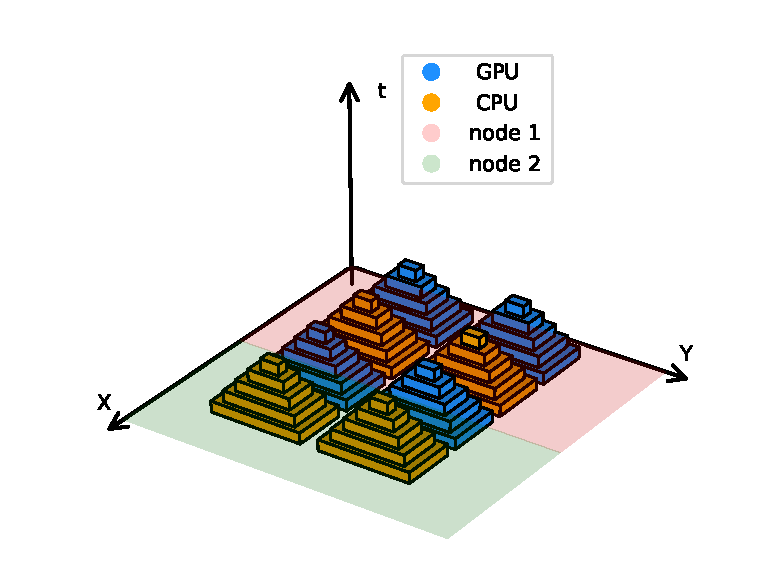
\includegraphics[scale=0.75, trim={1cm 0.6cm 0.5cm 0cm},,clip]{figs/UpPyramid1.pdf}
      \label{fig:Up-Pyramid}
    }
    \subfloat[\Yb{}: The subsequent phase of the swept solution process.]
    {
      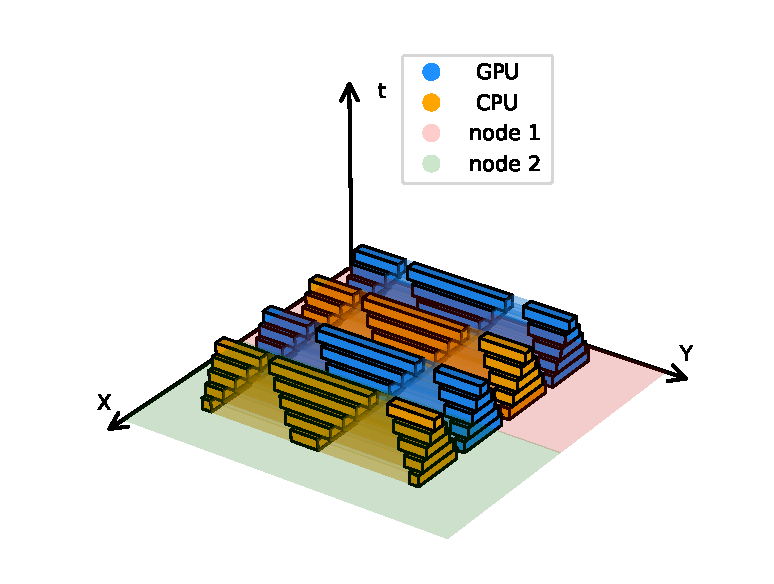
\includegraphics[scale=0.75, trim={1cm 0.6cm 0.5cm 0cm},clip]{figs/YBridge1.pdf}
       \label{fig:YBridge}
    }
    
    \subfloat[The first communication of the solution process.]
    {
      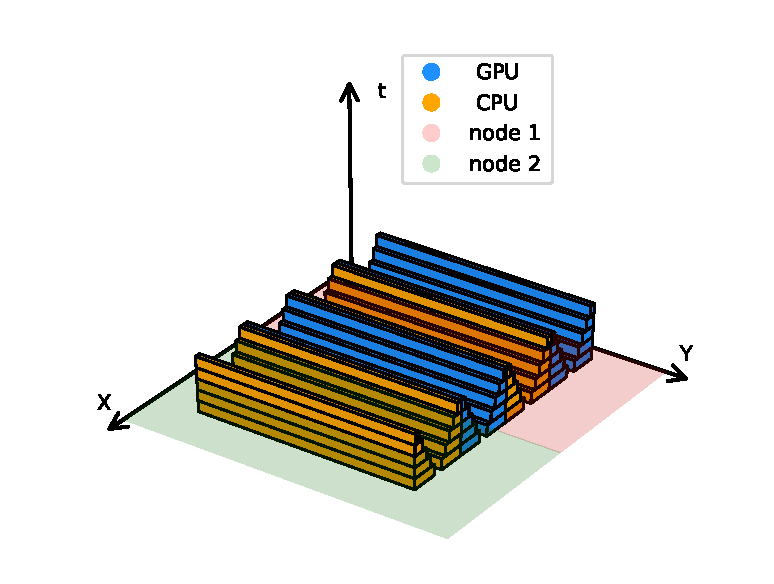
\includegraphics[scale=0.75, trim={1cm 0.6cm 0.5cm 0cm},,clip]{figs/Comm1.pdf}
       \label{fig:Comm1}
    }
    \subfloat[\Xb{}: The subsequent phase of the swept solution process.]
    {
      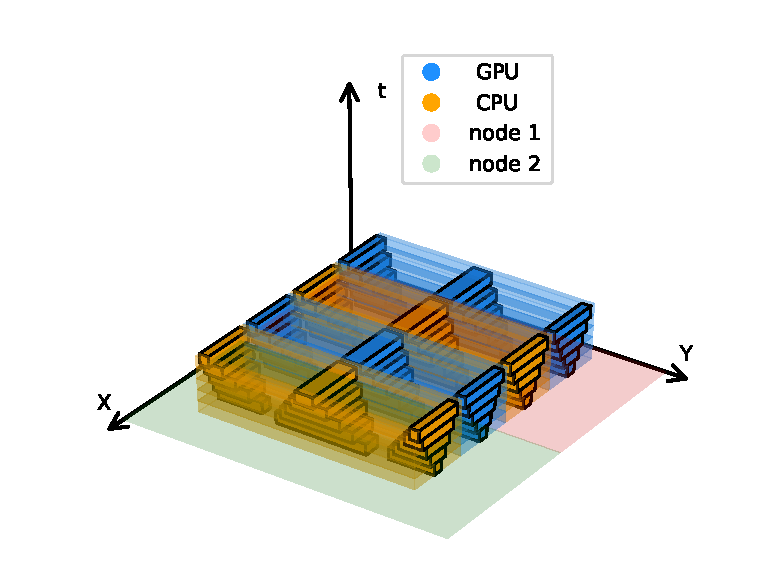
\includegraphics[scale=0.75, trim={1cm 0.6cm 0.5cm 0cm},,clip]{figs/XBridge1.pdf}
       \label{fig:Xbridge}
    }
    \caption{The first four steps in the swept solution process.}
    \label{fig:MainOne}
\end{figure}

\par
The first three phases in the swept solution process demonstrated in Figure~\ref{fig:MainOne} were followed by the \Oct{} phase shown in Figure~\ref{fig:Octahedron}. This phase is super position of the \Down{} and \Up{}. The \Down{}---shown in \ref{fig:Down-Pyramid}---always began with boundaries that were $2n$ and grew by $2n$ on each boundary with every passing time step. The  start was a natural consequence of removing these points during the \Up{} phase. The \Down{} was completed upon passing the top of the previous \Up{} or \Oct{} at which time the upward portion of \Oct phase began. The entire \Oct{} was calculated in the same fashion as the \Up{} on both CPU and GPUs. While the steps are described separately for clarity, they were performed in a single calculation step without communication between ranks. 

\par
The \Oct{} was always followed by the \Yb{}, Communicate, \Xb{} sequence. However, the communication varied in direction as the shift and communication of data was always the opposite of the former communication. We repeated this series of events as many times as was necessary to reach the final desired time of the simulation. The final phase is the aforementioned \Down{} which occurred only once at the end of the simulation. We show the ending sequence---minus the communication---in it's entirety in Figure~\ref{fig:MainTwo}. 
\par
To summarize the progression of swept phases, the \Up{} was calculated a single time; The Bridge and \Oct{} phases were then repeated until the simulation reached a value greater than or equal to that of the desired final time. The \Down{} was executed finally to fill in the remaining portion of the solution.

% Octahedron
\begin{figure}[!htb]
    \centering
    \subfloat[\Oct{}: An intermediate phase of the swept solution process.]
    {
      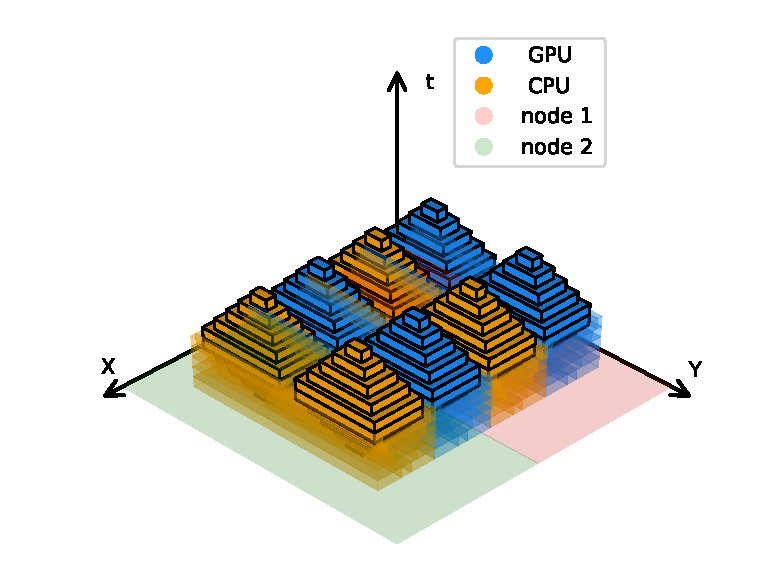
\includegraphics[scale=0.75, trim={1cm 0.6cm 0.5cm 0cm},clip]{figs/Octahedron1.pdf}
      \label{fig:Octahedron}
    }
    \subfloat[\Yb{}: The subsequent phase of the swept solution process.]
    {
      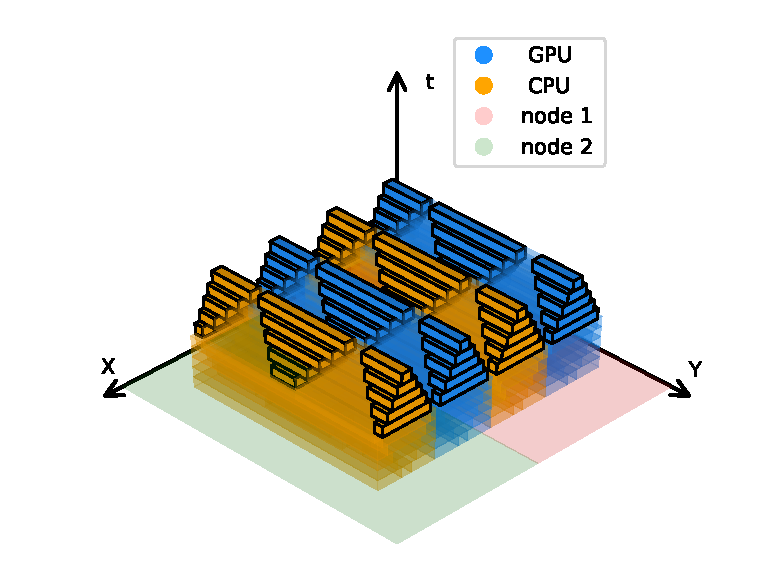
\includegraphics[scale=0.75, trim={1cm 0.6cm 0.5cm 0cm},clip]{figs/YBridge2.pdf}
       \label{fig:YBridge2}
    }

    \subfloat[\Xb{}: The next phase of the solution process.]
    {
      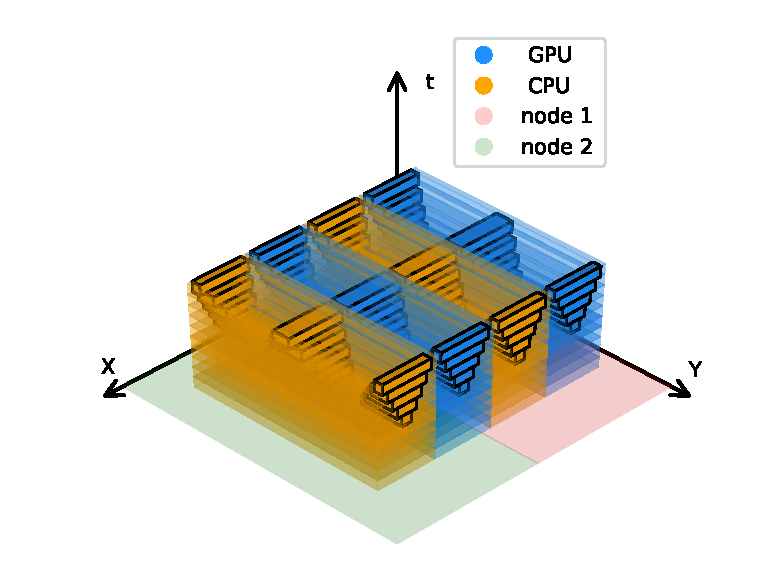
\includegraphics[scale=0.75, trim={1cm 0.6cm 0.5cm 0cm},,clip]{figs/XBridge2.pdf}
       \label{fig:XBridge2}
    }
    \subfloat[\Down{}: The final phase of the swept process.]
    {
      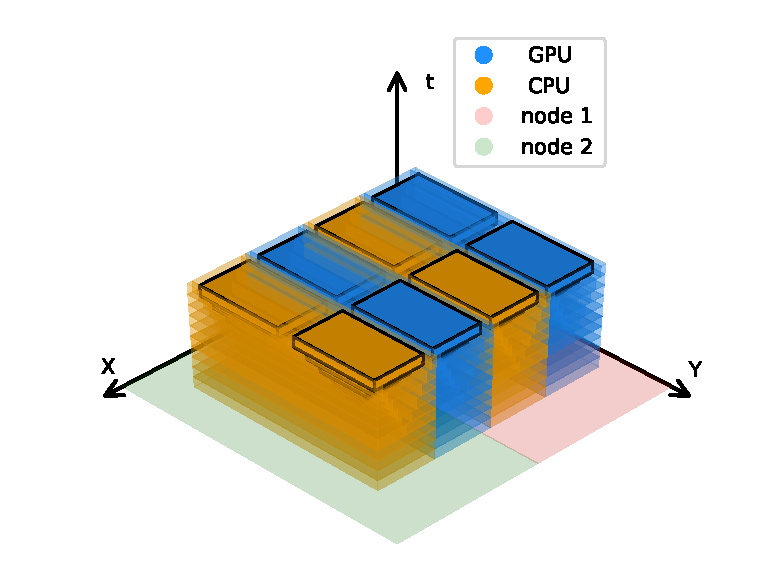
\includegraphics[scale=0.75, trim={1cm 0.6cm 0.5cm 0cm},,clip]{figs/DownPyramid1.pdf}
       \label{fig:Down-Pyramid}
    }
    \caption{The intermediate and final steps of the swept solution.}
    \label{fig:MainTwo}
\end{figure}

\par
The actual final time is determined by the number of swept steps, $S$, or the number of \Oct{} phases performed during simulation. This is determined by the given final time and $2h$, which is the minimum time possible of a simulation. It is this way because the simulation only stops after the completion of a phase. These phases occur on both the GPU and CPU with respect to the given share. In between each calculation step, a communication step occurs which consists of shared memory data management and writing to disk.

\par The shared memory data management of the communication step as well as the writing to disk involve a couple of nuances worth mentioning. It includes shifting of the data which is a strategy implemented for handling boundary blocks in the array. \pysweep{} was implemented with periodic boundary conditions based on the targeted test problems. The boundary blocks of the array form half of the shape it would normally in the direction orthogonal to the boundary (e.g. During the \Oct{} phase on the boundary where $x=0$, only half the \Oct{} will be formed in the x direction). As expected, the corner will form a fourth of the respective shape. In lieu of added logic for handling these varying shapes, a data shifting strategy was implemented which allows the majority of the same functions and kernels to be used. The boundary points are able to be solved as if they were in the center of a block with this strategy. This strategy comes at the expense of moving the data in memory. In hindsight, changing each processes perspective, i.e. the data it sees and manages, may be a more optimal way to implement this strategy.

\par \pysweep{} writes to disk during every communication as it is the ideal time. The code uses parallel HDF5 (h5py) so that each rank can write it's data to disk independently of other ranks \cite{Collette2008HDF5Python}. The shared memory array is the height of an \Oct{} in time plus the number of intermediate steps of the time scheme so that the intermediate steps of the scheme may be used for future steps if necessary. The appropriate fully solved steps are written to disk. The data is then moved down in the time dimension of the array and so that the next phase can be calculated in the existing space.

\par
In summary of this swept rule solution process, \pysweep{} is an extensible PDE solver that implements the swept rule in 2 dimensions on heterogeneous architecture. It consists of two primary steps which are calculation and communication. The calculation computes points based on a predictable patterns referenced as the phases of the simulation. The communication occurs after the \Yb{} forms along with shifting of the data so that the same logic may be used to calculated all of the points in the array. This shifting strategy provides simple communication logic at a minimal expense. The four phases---\Up{}, Bridge (X or Y), \Oct{}, and \Down{}---are the predictable shapes used to solve the problem in time. These shapes are available in Figures \ref{fig:MainOne} and \ref{fig:MainTwo}. 
\par
The solver has a few restrictions based on architecture and implementation which have been previously described. It is currently implemented for periodic boundary conditions but can be modified to suite other conditions using the same strategy. The solver is also capable of handling given CPU functions and GPU kernels so that it may be used for any desired application that falls within the guidelines presented here. \pysweep{} could certainly be further optimized but it is presently sufficient to test and determine the performance capabilities of the two dimensional heterogeneous swept rule in comparison to a traditional solver.

\section{Results}
\label{results-section}

\subsection{Heat Diffusion Equation}
\label{hdeResults}
The heat diffusion equation was solved numerically using Forward Euler in time and a three point central difference in space which gives the update formula shown in equation~\ref{heat-update}. We  validated the numerical solution against equation~\ref{heat-analyt}.
\begin{equation}
    \label{heat-update}
    T_{i,j}^{k+1} = T_{i,j}^{k}+\frac{\alpha \Delta t}{\Delta x^2}\big(T_{i+1,j}^{k}-2T_{i,j}^{k}+T_{i-1,j}^{k}\big)+\frac{\alpha \Delta t}{\Delta y^2}\big(T_{i,j+1}^{k}-2T_{i,j}^{k}+T_{i,j-1}^{k}\big)
\end{equation}
\begin{equation}
\label{heat-analyt}
    T(x,y,t) = sin(2\pi x)\,sin(2\pi y)\,e^{-8\pi^2\alpha t}
\end{equation}
The numerical and analytical solutions are graphically compared in figure~\ref{fig:heatSurface} and behave as expected.

\begin{figure}
    \centering
    \includegraphics{}
    \caption{Heat Diffusion}
    \label{fig:heatSurface}
\end{figure}

We measured performance of the swept rule applied to the heat diffusion equation by speed up of the swept rule, $S$, as a function of array size, block size, and share is found based on the run time, $R_i$, of a simulation $i$. 
\begin{equation}
    S = \frac{R_{standard}}{R_{swept}}
\end{equation}
The performance results produced by these simulations are shown in Figures~\ref{fig:newSpeedup} and~\ref{fig:oldSpeedup} for the two sets of hardware as described in section~\ref{parameters-section}. 
A third contour of speedup is shown in Figure~\ref{fig:heatHardwareComp} to compare the performance across  the differing hardware. This speed up is found as $R_{swept,2}/R_{swept,1}$. In these figures, a black dot with a white border represents the optimal case and a white dot with a black border represents the worst case. Finally, this section is concluded with Figure~\ref{fig:heatTimeStep} which presents $S$ for both sets of hardware as a function of the number of time steps. 

\begin{figure}[htb!]
    \centering
    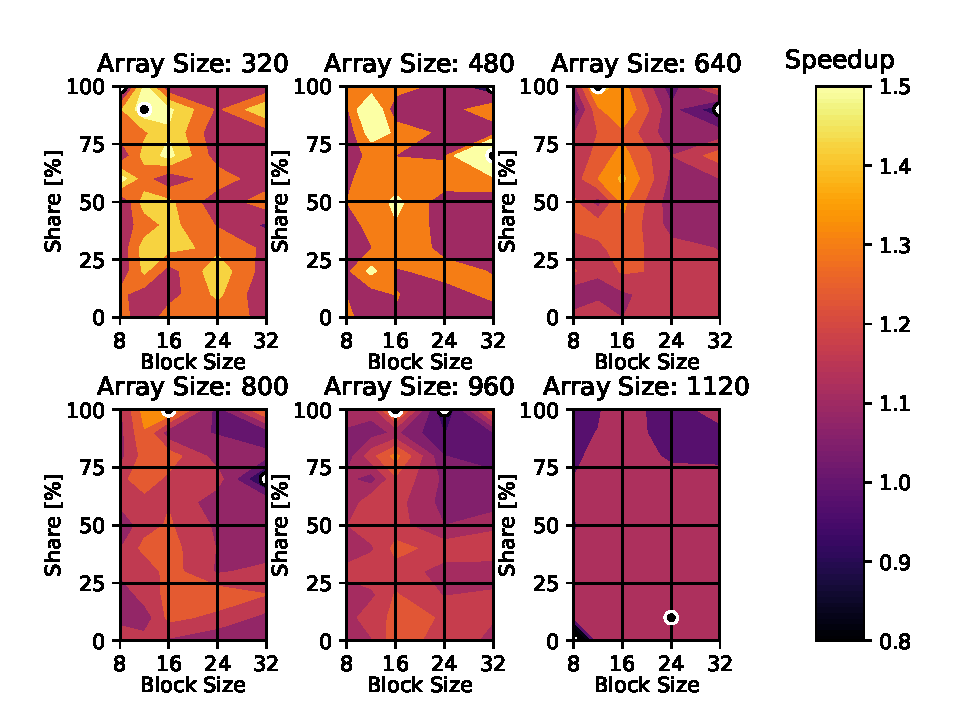
\includegraphics[scale=0.7]{figs/speedUpheatNew.pdf}
    \caption{Swept rule speed up results with \newGPU{} GPUs and \newCPU{} CPUs.}
    \label{fig:newSpeedup}
\end{figure}

In Figure~\ref{fig:newSpeedup} it is clear that the performance of the swept rule diminishes as the array size is increased. However, it does seem to approach a limit to this decrease on the maximum array size. Shares greater than approximately 70\% seem to contain the best as well as the worst cases. It also seems that better performance is obtained by lower block sizes.

\begin{figure}[htb!]
    \centering
    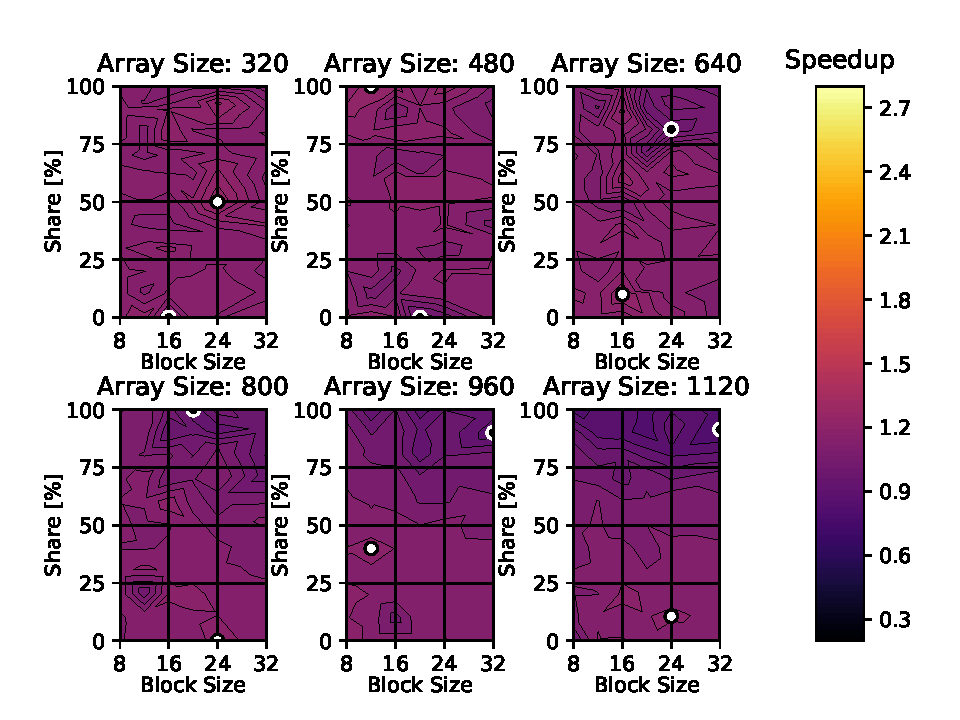
\includegraphics[scale=0.7]{figs/speedUpheatOld.pdf}
    \caption{Swept rule speed up results with \oldGPU{} GPUs and \oldCPU{} CPUs.}
    \label{fig:oldSpeedup}
\end{figure}

In Figure~\ref{fig:oldSpeedup}, we see some differing trends than Figure~\ref{fig:newSpeedup}. The array size trend holds but trends based on the other two parameters are unclear. It seems that performance is better with lower shares in the case of this hardware and somewhat consistent across different block sizes. 

\begin{figure}[htb!]
    \centering
    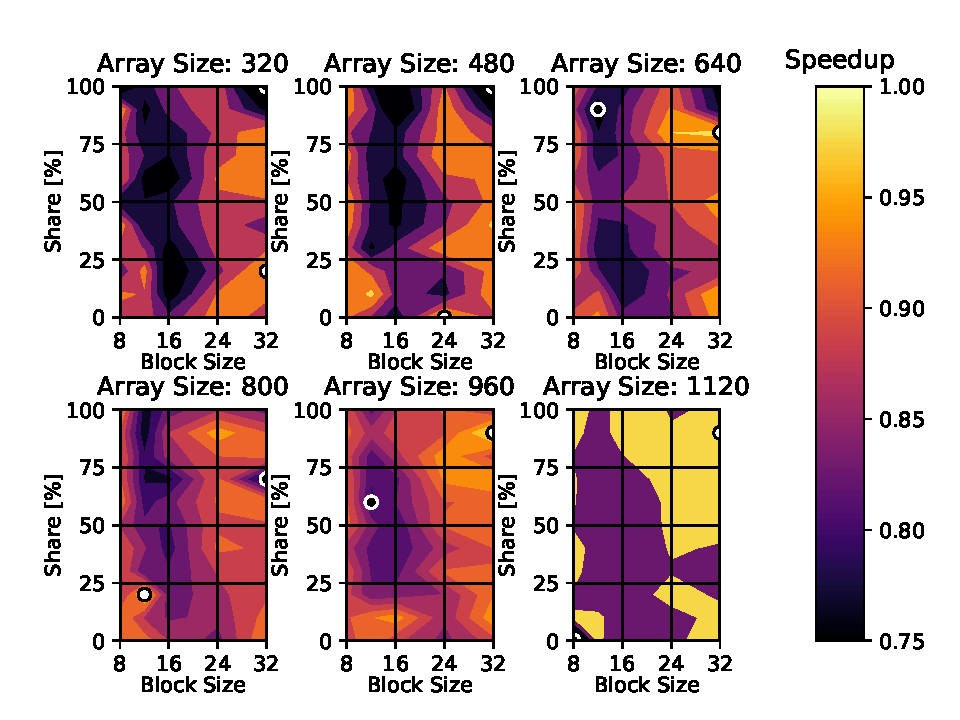
\includegraphics[scale=0.7]{figs/hardwareSpeedupHeat.pdf}
    \caption{Hardware speed up comparison for the heat diffusion equation.}
    \label{fig:heatHardwareComp}
\end{figure}

In Figure~\ref{fig:heatHardwareComp} we see that hardware set one is consistently slower than hardware set two---at best it is equivalent. It seems to be particularly worse at lower block sizes over a large range of shares. Specifically, shares of 25\% to 100\% are the worst.

\begin{figure}
    \centering
    \includegraphics{}
    \caption{Caption}
    \label{fig:heatTimeStep}
\end{figure}

\subsection{Compressible Euler's Equations}
\label{eulerVortexResults}


\subsection{Hardware Comparison}
\label{hardwareResults}

\section{Discussion}
\label{discussion-section}
In regards to the heat diffusion equation, we see an overall range of speed up from 


\section{Conclusions}
\label{conclusions-section}



\section{Acknowledgements}
This material is based upon work supported by NASA under award No. NNX15AU66A under the technical monitoring of Drs. Eric Nielsen and Mujeeb Malik. We also gratefully acknowledge the support of NVIDIA Corporation, who donated a
Tesla K40c GPU used for this research.

\bibliographystyle{unsrt}
\bibliography{references}

\section{Appendix}
\label{appendices}
\subsection{Numerical Problems}
\subsubsection{Heat Diffusion Equation}
\subsubsection{Euler Vortex}

\label{AppendixA}
\subsection{Hardware}
\label{AppendixB}
\begin{table}[htb!]
\begin{center}
\begin{tabular}{ |c|c|c| } 

 \hline
 Hardware Specifications & Set 1 & Set 2 \\ 
 \hline
 GPU & \newGPU{} & \oldGPU{} \\
 Architecture   & Volta &  Pascal \\
 NVIDIA CUDA® Cores  & 5120 &  3584 \\
 Memory Type   & 32 GB HBM2 &  11 GB GDDR5X \\
 Bus Width    & 4096 bit &  352-bit \\
 Memory Bandwidth (GB/sec)  & 900 &  484 \\ 
 \hline
 CPU & \newCPU{} & \oldCPU{} \\ 
 Cores & 20 & 10 \\
 Processor Base Frequency & 2.20 GHz & 2.20 GHz \\
 Cache & 50 MB Intel® Smart Cache & 13.75 MB L3 Cache\\
 \hline
\end{tabular}
\end{center}
\caption{\label{hardwareTable} Common specifications found between hardware sets from NVIDIA's and Intel's websites \cite{Intel123550,Intel91753,NVIDIANVIDIA,GeForceGeForce}.}
\end{table}
\end{document}
